\documentclass[11pt]{article}

% -------------------------------------------------
% PACKAGES
% -------------------------------------------------
\usepackage[letterpaper,margin=1in]{geometry}
\usepackage{amsmath, amssymb, amsthm}
\usepackage{graphicx, xcolor, multirow, enumerate, fancyhdr, caption, listings, wrapfig}
\usepackage{tikz, pgfplots}
\usetikzlibrary{calc, arrows.meta, positioning, decorations.markings, shadings}
\usepackage{booktabs}
\usepackage{authblk} % for multiple authors
\usepackage{lipsum}
\usepackage{hyphenat}
\usepackage{float}
\usepackage[colorlinks=true, urlcolor=black, linkcolor=black]{hyperref}


% -------------------------------------------------
% CODE SETTINGS
% -------------------------------------------------
\lstset{
  language=Matlab,
  basicstyle=\ttfamily\small,
  keywordstyle=\color{blue},
  stringstyle=\color{violet},
  commentstyle=\color{teal},
  frame=single,
  framesep=10pt,
  xleftmargin=10pt,
  xrightmargin=10pt,
  breaklines=true,
  numbers=left,
  numberstyle=\tiny\color{gray},
  showstringspaces=false,
  tabsize=4,
  captionpos=b
}

% -------------------------------------------------
% TITLE BLOCK
% -------------------------------------------------
\title{\vspace{-1.2cm} % move title up
\bfseries\Large Multimodal Alpha Forecasting and Robust Portfolio Optimization}

\author[]{Catherine Ma (\texttt{cama12@mit.edu})}
\author[]{Hanna Zhang (\texttt{zeyuzh@mit.edu})}
\affil[]{}

\date{} % hide date completely

% -------------------------------------------------
% DOCUMENT
% -------------------------------------------------
\begin{document}
% \begin{titlepage}
%     \centering
%     \vspace*{3cm}

%     {\Large \textbf{15.095 Machine Learning Under a Modern Optimization Lens}}\\[1.2 cm]
%     {\large \textbf{Multimodal Alpha Forecasting and Robust Portfolio Optimization}}\\[1.2cm]

%     {\large Catherine Ma (cama12@mit.edu) \& Hanna Zhang (zeyuzh@mit.edu)}\\[0.5cm]
%     {\large May 30, 2025}

%     \vfill
% \end{titlepage}
\begin{titlepage}
  \begin{center}
    \vspace*{\fill}

    {\huge \textit{15.095 Machine Learning Under a Modern Optimization Lens}}

    \vspace{0.5cm}

    {\huge \textbf{Multimodal Alpha Forecasting and Robust Portfolio Optimization}}

    \vspace{1.5cm}

    {\Large \textbf{Catherine Ma (\texttt{cama12@mit.edu}) \& Hanna Zhang (\texttt{zeyuzh@mit.edu})}}\\

    \vspace*{\fill}
  \end{center}
\end{titlepage}

% \begin{abstract}
%     ............To be completed............
% \end{abstract}

\section{Introduction}
\noindent Short-horizon equity return prediction is one of the most challenging problems in quantitative finance. 
Daily returns have extremely low signal-to-noise ratios, are influenced by market microstructure noise, and arise from nonlinear macro, sector, and firm-level drivers.
Despite this difficulty, even marginal improvements in predictive accuracy can lead to economically meaningful gains when integrated into a risk-controlled portfolio optimization framework. \\

\noindent The goal of this project is to develop a multimodal forecasting system that integrates diverse sources of information: price-based technical indicators, firm fundamentals, macroeconomic variables, sector classifications, calendar effects, and sentiment signals and text embeddings from news data. 
We aim to evaluate which feature groups contribute meaningful predictive power and generate a next-day return forecast suitable for prescriptive portfolio optimization.

\section{Data}

\subsection{Data Sources}
To support our modeling framework, we compile a daily panel for S\&P~500 stocks using information from multiple independent datasets:
\begin{itemize}
    \item \textbf{S\&P 500 Constituents:}  
    List of S\&P~500 tickers used to define the modeling universe.

    \item \textbf{Stock Market Data:}  
    Daily OHLCV (Open, High, Low, Close, Volume) prices for all S\&P~500 stocks from 2016--2023 from Yahoo Finance.

    \item \textbf{Company Fundamentals:}  
    Firm-level financial metrics, such as profitability, margins, growth, leverage, and valuation ratios, sourced from WRDS/Compustat.

    \item \textbf{Macroeconomic Indicators:}  
    FRED variables, including interest rates, GDP growth, unemployment rates, and treasury yields. 

    \item \textbf{News Data:}  
    Daily financial news headlines and summaries collected from the FNSPID datasetm used to compute sentiment scores and text embeddings.\footnote{\url{https://huggingface.co/datasets/Zihan1004/FNSPID}}
\end{itemize}

\subsection{Data Processing Pipeline}
All data are merged at the (ticker, date) level to form a consistent daily panel. The main steps are:

\begin{enumerate}
    \item \textbf{Cleaning and Alignment:}  
    All data sources are standardized to daily frequency. To avoid look-ahead bias, missing fundamental values are forward-filled within each firm.

    \item \textbf{Target Variable:}  
    The next-day return is computed from daily closing prices and used as the prediction target.

    \item \textbf{Feature Engineering:}  
    We generate four major classes of predictors:
    \begin{itemize}
        \item \textbf{Price-Based Technical Features:} 
        Multi-horizon moving averages, exponential moving averages, rolling-window returns, log volume, and other short-term indicators.
        
        \item \textbf{Fundamental Features:} 
        Profitability metrics (ROA, ROE), margins (gross, operating, and net margins), growth rates, valuation ratios (book-to-market, earnings yield, cash-flow yield), and balance-sheet indicators (leverage, liquidity, cash holdings).
        
        \item \textbf{Macroeconomic Variables:} 
        VIX, yield curve spreads, Fed Funds Rate, industrial production, unemployment, GDP, and other broad economic indicators.
        
        \item \textbf{Text Features:}
        Sentiment scores derived from FinBERT (positive, negative, neutral classifications aggregated into daily measures such as mean sentiment, extremal sentiment, and news count), and 768-dimensional FinBERT text embeddings obtained from headlines and summaries and averaged within each stock-day to capture linguistic tone and narrative content.
        
        \item \textbf{Dimension Reduction:}
        High-dimensional text embeddings are compressed into 64 components via PCA, preserving most of the variance while~reducing~computational~cost.

        \item \textbf{Sector and Time Structure:}
        One-hot sector and subsector classifications, plus day-of-week and month-of-year dummies capturing calendar seasonality.
    \end{itemize}


    % \item \textbf{Handling Missing Values:}  
    % \begin{itemize}
    %     \item \emph{Forward-filling time-invariant}  
    %     (e.g., fundamentals such as leverage, ROA, and margins).  
    %     These variables are forward-filled \emph{within each firm} so that only past information is used, which prevents look-ahead bias.

    %     % \item \emph{Zero-filling structurally missing ratios or indicators}  
    %     % (e.g., variables undefined for certain firms or years).  
    %     % This approach preserves the panel structure without imputing information from the future.
    % \end{itemize}

    \item \textbf{Train--Validation--Test Split:}  
    The data is segmented chronologically into:
    \[
    \text{Train: 2016--2021},\quad
    \text{Validation: 2022},\quad
    \text{Test: 2023}.
    \]
    This prevents information leakage and ensures realistic out-of-sample evaluation.

\end{enumerate}

\noindent The resulting dataset provides a multimodal view of cross-sectional and time-series drivers of equity behavior, providing a basis for evaluating the predictive contribution of different feature families.

\section{Methodology}
\subsection{Stock Next Day Return Prediction}
\subsubsection*{Evaluation Metric}
Because the goal is to forecast next-day equity returns in a noisy, low-signal environment, the evaluation framework must reflect practical trading considerations. Although models output real-valued return forecasts, the primary operational question is whether the model correctly anticipates the \emph{direction} of the next day's movement, as this determines the trading position taken.

\vspace{6pt}
\noindent To align with this objective, we use \textbf{Directional Accuracy (DA)} as the evaluation metric. DA measures the fraction of predictions whose sign matches the sign of the realized next-day return:

\[
\text{DA} = \frac{1}{N} \sum_{i=1}^{N} \mathbf{1}\left\{\, \operatorname{sign}(\hat{r}_i) = \operatorname{sign}(r_i) \,\right\},
\]


\noindent where $\hat{r}_i$ is the predicted next-day return and $r_i$ is the realized next-day return. A DA of $50\%$ corresponds to random guessing in a balanced up/down environment, so even small improvements (1--2 percentage points) are economically meaningful.

% TO UPDATE THE MODELS SECTION BELOW 
\subsubsection{Baseline Models}

% \begin{figure}[ht]
%     \centering
%     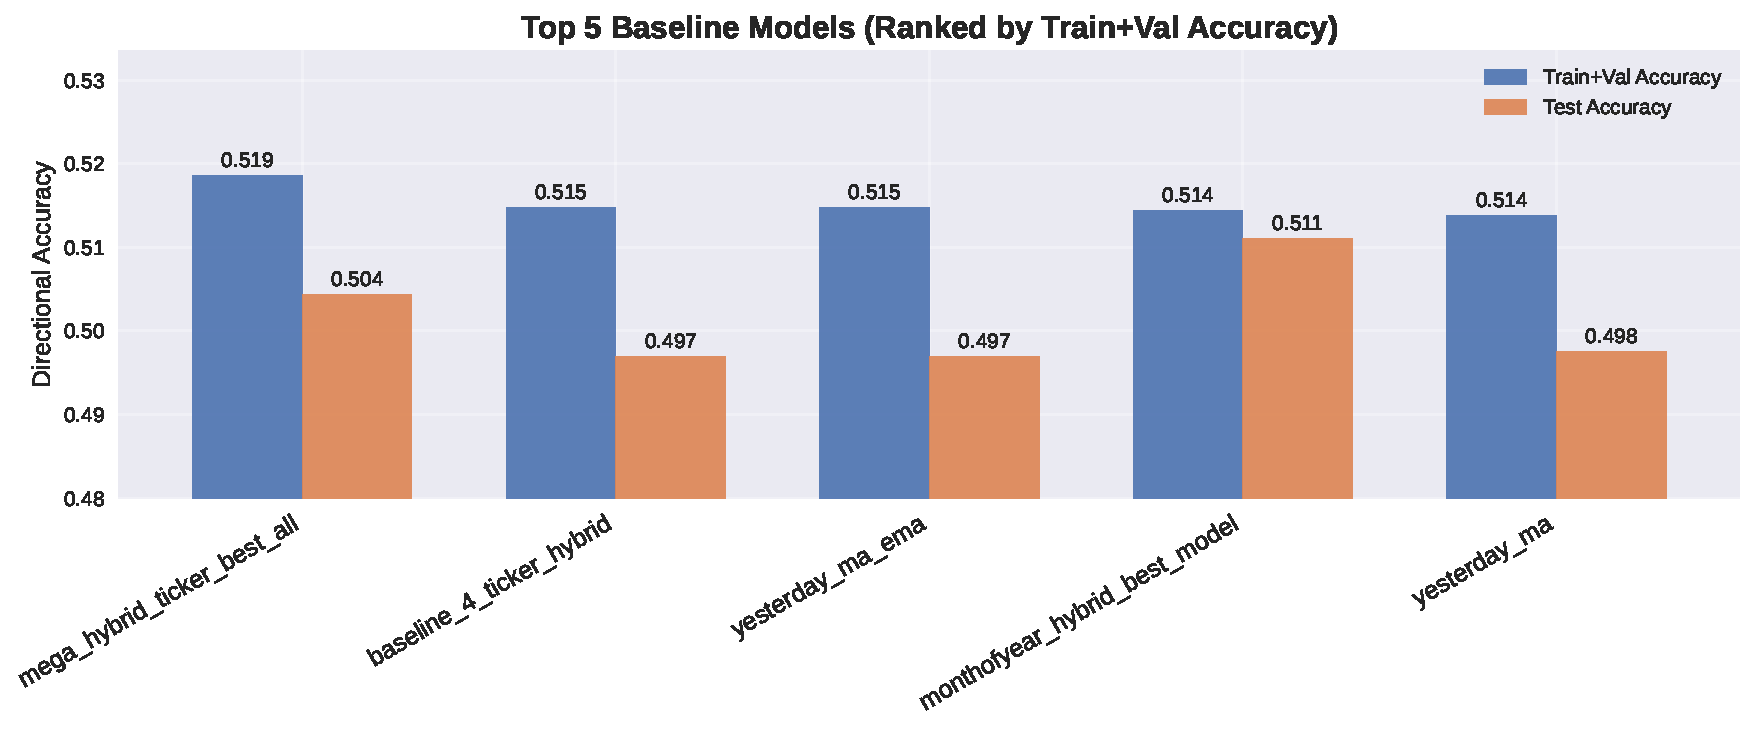
\includegraphics[width=0.9\linewidth]{../figures/baseline_model_comparison_top5.pdf}
%     \caption{\textbf{Top 5 baseline models ranked by train+validation accuracy.}}
%     \label{fig:top5_baseline}
% \end{figure}

Before introducing flexible machine learning methods, we construct a suite of simple, 
deterministic forecasting rules. These baselines serve two purposes:  
(i) to provide interpretable benchmarks grounded in standard quantitative finance heuristics 
(e.g., momentum and seasonality), and  
(ii) to quantify how much apparent predictability can arise from rule selection rather than 
genuine signal.

\noindent All baseline models are evaluated on the same S\&P~500 daily return panel using the 
2016--2022 train--validation period and the 2023 test set.

\subsubsection*{Single-Rule Baselines}

These models apply the same fixed rule across all stocks and dates:

\begin{itemize}
    \item \textbf{Naive persistence:} predicts tomorrow's return as today's return.
    \item \textbf{Moving averages (MA):} simple averages over windows such as 2--60 days.
    \item \textbf{Exponential moving averages (EMA):} exponentially weighted versions of MA rules.
    \item \textbf{Seasonal rules (S1--S7):} include same-day-last-year, same-month-last-year, 
    month-of-year means, day-of-week means, and rolling long-horizon averages (21-day, 63-day).
\end{itemize}

\noindent Directional accuracy for these rules generally clusters around 50\%.  
The persistence rule performs at chance, short-horizon MA/EMA rules yield modest improvements 
(50.2--50.5\% in-sample, reverting toward 50\% on test), and several seasonal rules stand out.  
The day-of-week mean achieves roughly 50.6\% train--validation accuracy and 50.9\% on the test set, 
and the month-of-year mean reaches nearly 52\% on test, suggesting that coarse calendar structure 
generalizes better than aggressively tuned short-term momentum rules.

\subsubsection*{Hybrid Baselines}

To relax the ``one-rule-for-all'' constraint, we evaluate hybrid baselines that allow different 
segments of the data to select their own preferred single-rule predictor based on 
2016--2022 performance:

\begin{itemize}
    \item \textbf{Per-ticker:} each stock selects its best single-rule baseline.
    \item \textbf{Per-month:} each calendar month selects its best rule.
    \item \textbf{Per-day-of-week:} each weekday selects its best rule.
\end{itemize}

\begin{center}
\begin{tabular}{lcc}
\toprule
\textbf{Hybrid Method} & \textbf{Train+Val DA} & \textbf{Test DA} \\
\midrule
Per-ticker   & 0.5185 & 0.5044 \\
Per-month    & 0.5144 & 0.5110 \\
Per-day-of-week & 0.5119 & 0.5040 \\
\bottomrule
\end{tabular}
\end{center}

\noindent The per-ticker method attains the highest in-sample accuracy but does not generalize well, 
while the month-of-year hybrid yields the most stable out-of-sample performance.  
Notably, the hybrid selections reveal recurring patterns: the day-of-week average is chosen 
for 143 tickers, long-horizon rolling means for 59, and several MA/EMA windows (50-day EMA, 
1-month, 3-day, 14-day) are frequently selected.  
These patterns indicate that calendar structure and slower-moving return components are the 
most consistently useful simple predictors, and they inform which feature families are emphasized 
in the subsequent machine learning models.

\subsubsection*{Summary}

Overall, the baseline results confirm that next-day return prediction is extremely noisy:  
simple rules rarely exceed 51\% accuracy.  
Nonetheless, seasonality and long-horizon momentum effects provide weak but persistent signals 
that serve as meaningful benchmarks for evaluating more flexible multimodal models.



\subsubsection{XGBoost}
\subsubsection{CatBoost}
\subsubsection{LightGBM}

\section{Baseline Models}

We first construct a suite of deterministic baseline models applied uniformly across tickers:

\subsection{Single-Rule Baselines}

\begin{itemize}
    \item \textbf{Persistence}: $\hat{r}_{t+1} = r_t$
    \item \textbf{Moving Averages}: 3--63 day averages.
    \item \textbf{Exponentially Weighted MAs}: EMA windows for momentum smoothing.
    \item \textbf{Seasonal Rules (S1--S7)}:
    \begin{itemize}
        \item Same-day-last-year
        \item Same-month-last-year
        \item Month-of-year mean
        \item Day-of-week mean
        \item Long-horizon (21/63-day) rolling means
    \end{itemize}
\end{itemize}

Results show DA values clustered near 50\%, with the strongest being the day-of-week and month-of-year seasonal patterns (up to $52\%$ DA on test).

\subsection{Hybrid Baselines}

We also allow simple rules to vary across segments:

\begin{itemize}
    \item \textbf{Per-Ticker}: choose best-performing baseline for each stock.
    \item \textbf{Per-Month}: choose best baseline for each calendar month.
    \item \textbf{Per-Day-of-Week}: choose best baseline for each weekday.
\end{itemize}

The per-ticker hybrid achieves the highest validation accuracy ($\approx 0.518$), though generalization remains limited ($\approx 0.504$ test).  
The most frequently chosen signals were:
\begin{itemize}
    \item Day-of-week seasonal rule (selected for 143 tickers)
    \item Long-horizon rolling means (59 tickers)
    \item MA and EMA windows (various)
\end{itemize}

This motivates the engineered price features in the next stage.

\section{Price-Only Machine Learning Models}

\subsection{Engineered Signal Features}

We construct price-based features closely aligned with patterns favored by the hybrid baselines:

\begin{itemize}
    \item Lagged returns ($b0$)
    \item Moving averages: 2d, 1w, 2w, 1m, 30d, 50d
    \item Rolling drift indicators (21d, 63d)
    \item Seasonal means: day-of-week, month-of-year
\end{itemize}

These features form the \textbf{signal design matrix} for subsequent modeling.

\subsection{Models Trained}

\begin{itemize}
    \item Linear Regression
    \item XGBoost (baseline configuration)
    \item XGBoost (grid-tuned)
    \item KNN Regression
    \item Support Vector Regression
    \item Neural Network with ticker embeddings
\end{itemize}

\subsection{Key Findings}

\begin{itemize}
    \item Linear regression achieves roughly 50--51\% DA.
    \item XGBoost outperforms linear models, reaching $\approx 0.528$ on validation and $\approx 0.509$ on test.
    \item KNN and SVR underperform due to high dimensionality and noise.
    \item Neural networks with ticker embeddings improve slightly but remain below tuned boosting models.
    \item Ablation studies show that a compact subset of \textbf{seasonality + long-horizon drift} features nearly matches the full model.
\end{itemize}

\section{Core Structural Features}

We introduce categorical and structural features:

\begin{itemize}
    \item Day-of-week (one-hot)
    \item Month-of-year (one-hot)
    \item Sector and subsector (from S\&P 500 metadata)
    \item Volume and log-volume
\end{itemize}

Models trained on these features include linear regression, XGBoost, and LightGBM.

The structural feature set consistently outperforms pure price-only:  
tuned XGBoost reaches $\approx 0.521$ validation DA.

\section{Combining Signals and Structural Features}

We build a \textbf{signal + core} feature matrix including both engineered price signals and structural variables.  
Across linear models, boosting methods, and neural networks, combined features consistently outperform either family alone.

\subsection{DOW + Month + Sector as a Core Predictor Set}

Ablations reveal that the following three groups carry the most robust signal:

\[
\text{Day-of-Week} \;+\; \text{Month-of-Year} \;+\; \text{Sector}
\]

This ``DMS'' set becomes the foundation for the final modeling stage.

\section{Extending DMS With Fundamentals, Macro, Sentiment, and PCA Embeddings}

Let $DMS$ denote the union of day-of-week, month, and sector dummies.  
We extend DMS using the following families:

\subsection{Fundamental Features}

\begin{itemize}
    \item Growth: sales\_growth\_qoq, sales\_growth\_ttm, asset\_growth
    \item Profitability: roa\_ttm, roe\_ttm
    \item Margins: gross / operating / net margin
    \item Valuation: log\_mktcap, bm, earnings\_yield, cf\_yield, sales\_yield, div\_yield
    \item Balance sheet: leverage, current\_ratio, cash\_assets, accruals\_ta
\end{itemize}

\subsection{Macroeconomic Features}

\begin{itemize}
    \item Inflation, Fed Funds, GDP, unemployment
    \item Treasury yields (10y, 2y, 3m), corporate yield (AAA)
    \item VIX, S\&P 500 index, yield spread 10y--2y
\end{itemize}

\subsection{Sentiment Features}

\begin{itemize}
    \item mean, max, min, sum sentiment
    \item news count
\end{itemize}

\subsection{Text Embeddings}

\begin{itemize}
    \item PCA-reduced text embeddings: pca\_emb\_*
\end{itemize}

\section{Best Models (From Final Notebook)}

We evaluate LightGBM with the following feature subsets:

\subsection{Model A: Best Validation DA}

LightGBM trained on:

\[
\text{DMS} + \{\log\_mktcap, bm, earnings\_yield, cf\_yield, roa\_ttm, roe\_ttm\}
\]

Achieves:
\[
    \mathrm{Val\,DA} \approx 0.522
\]

\subsection{Model B: Best Test DA}

LightGBM trained on:

\[
\text{DMS} + \{\text{mean\_sentiment}\}
\]

Achieves:
\[
    \mathrm{Test\,DA} \approx 0.540
\]

\section{Conclusion}

Across more than a dozen modeling configurations, several themes emerge:

\begin{itemize}
    \item Pure price-derived signals carry weak but usable predictive structure.
    \item Core structural features, particularly day-of-week, month-of-year, and sector, are consistently predictive.
    \item Combining signals with structural variables improves performance.
    \item Adding fundamentals and sentiment on top of DMS leads to further gains.
    \item LightGBM and CatBoost outperform linear models, XGBoost, and neural networks on this tabular data.
    \item The strongest model tested was LightGBM using \textbf{DMS + mean sentiment}, achieving $\approx 0.54$ test directional accuracy.
\end{itemize}


\subsection{Robust Portfolio Optimization}

While predictive accuracy indicates that the model captures return-relevant
patterns, turning point forecasts into actionable trades requires an allocation
rule that respects risk, diversification, and transaction costs. Simple
heuristics such as equal-weighting or top-$K$ selection ignore downside
exposures and often produce unstable, overly concentrated portfolios whose
performance exaggerates the value of the underlying signal.\\

\noindent To obtain realistic and risk-aware allocations, we employ a robust
Conditional Value-at-Risk (CVaR) optimization layer. CVaR determines the weight
assigned to each equity by evaluating how the portfolio would behave under a
rolling set of recent historical return scenarios. For each day’s prediction
vector, the optimizer searches for weights that increase exposure to stocks with
high predicted returns, but penalize those that contribute heavily to losses in
the worst tail of the return distribution. In practice, this yields portfolios
that favor assets with both attractive forecasts and stable downside behavior,
while enforcing constraints such as long-only positions, position-size caps, and
turnover limits. The result is a set of portfolio weights that are smoother,
more diversified, and more robust than those produced by naïve allocation
rules.

\subsubsection{CVaR Formulation}
Rather than relying on variance as a proxy for risk, we use CVaR to focus directly on large downside losses. CVaR measures
the expected loss in the worst $(1-\alpha)$ fraction of outcomes and remains
well-behaved even when returns are skewed or heavy-tailed. Given portfolio weights $w$ and a set of recent scenario returns
$\{r_t\}_{t=1}^{T}$, CVaR at confidence level $\alpha = 0.95$ is written using
auxiliary variables $v$ (the VaR cutoff) and $z_t$ (tail losses):
\[
\mathrm{CVaR}_{\alpha}(w)
    = v + \frac{1}{(1-\alpha)T}
      \sum_{t=1}^{T} z_t,
\qquad
z_t \ge 0,\quad
z_t \ge -(r_t^\top w) - v.
\]
This linear representation makes the CVaR objective directly optimizable.

\subsubsection{Rolling Scenario Construction}
The scenario matrix is built from the most recent 60 days of realized
cross-sectional returns. Using a rolling window allows the optimizer to reflect
current market conditions---including changes in volatility, correlations, and
downside risk—without assuming a particular return distribution. As market
regimes shift, the CVaR optimizer naturally updates its estimate of tail risk
and adjusts portfolio weights accordingly.


\subsubsection{Optimization Objective and Constraints}
At each date $t$, the optimizer selects weights for each equity by solving
\[
\max_{w}
\quad
\hat{\mu}_t^\top w
\;-\;
\lambda\, \mathrm{CVaR}_{0.95}(w)
\;-\;
\mathrm{TC} \cdot \| w - w_{t-1} \|_1,
\]
\noindent where $\hat{\mu}_t$ are the model's predicted next-day returns (scaled for
numerical stability), $\lambda$ controls aversion to tail risk, and the
$\ell_1$ turnover term penalizes excessive rebalancing and incorporates
proportional transaction costs. \\

\noindent We impose the following practical trading constraints:
\begin{itemize}
    \item \textbf{Long-only and fully invested:}
          $w_i \ge 0$, $\sum_i w_i = 1$.
    \item \textbf{Position limit:}
          $w_i \le 2\%$ to prevent concentration.
    \item \textbf{Turnover limit:}
          $\|w - w_{t-1}\|_1 \le 10\%$ to avoid hyperactive trading.
    \item \textbf{Transaction cost penalty:}
          proportional cost of 5 bps per unit turnover.
\end{itemize}
These constraints make the optimization problem both realistic and stable,
preventing extreme weight allocations that often arise in unconstrained ML
portfolios.

\subsubsection{Backtesting Procedure}
For each model's cross-sectional predictions, we build a $T \times N$ matrix of
predicted returns and a matching matrix of realized one-day-ahead returns. The
portfolio is rebalanced daily using the CVaR optimizer. Performance is reported
using standard metrics:
\[
\text{Sharpe ratio},\quad
\text{annualized return},\quad
\text{annualized volatility},\quad
\text{and maximum drawdown}.
\]

\noindent Importantly, CVaR-based optimization acts as a ``stress test'' for the machine
learning signals: only predictions that are stable, consistent across the
cross-section, and resistant to noise will survive the downside-risk penalty
and turnover constraints.

\section{Results}
To compare the predictive contribution of different input modalities, we evaluate five LightGBM models trained on progressively richer feature sets:

\begin{itemize}
    \item \textbf{Fundamentals:} Day-Month-Sector (DMS), log market capitalization ($\log\_mktcap$), book-to-market ratio (bm), return on assets ($\text{roa\_ttm}$), and return on equity ($\text{roe\_ttm}$).
    \item \textbf{Mean Sentiment:} DMS, and mean sentiment score from news data.
    \item \textbf{Mean Sentiment + Embeddings:} DMS, mean sentiment score, and text embeddings.
    \item \textbf{News Momentum:} DMS and a full set of leak-free sentiment momentum predictors.  
    For each raw sentiment variable $f \in \{\text{mean},\text{max},\text{min},\text{sum},\text{count}\}$,  
    the feature set includes:
    $f$, $f_{\text{lag1}}$, $f_{\text{roll3}}$, $f_{\text{roll5}}$, $f_{\text{vol5}}$, $f_{\text{shock}}$, and $f_{\text{surprise3}}$.
    \item \textbf{News Momentum + Embeddings:} DMS, News Momentum, and text embeddings.

\end{itemize}

\subsection*{Directional Accuracy for LightGBM Models with Different Feature Sets}
\begin{figure}[H]
    % \hspace*{-1.5cm} % adjust horizontal position
    \center
    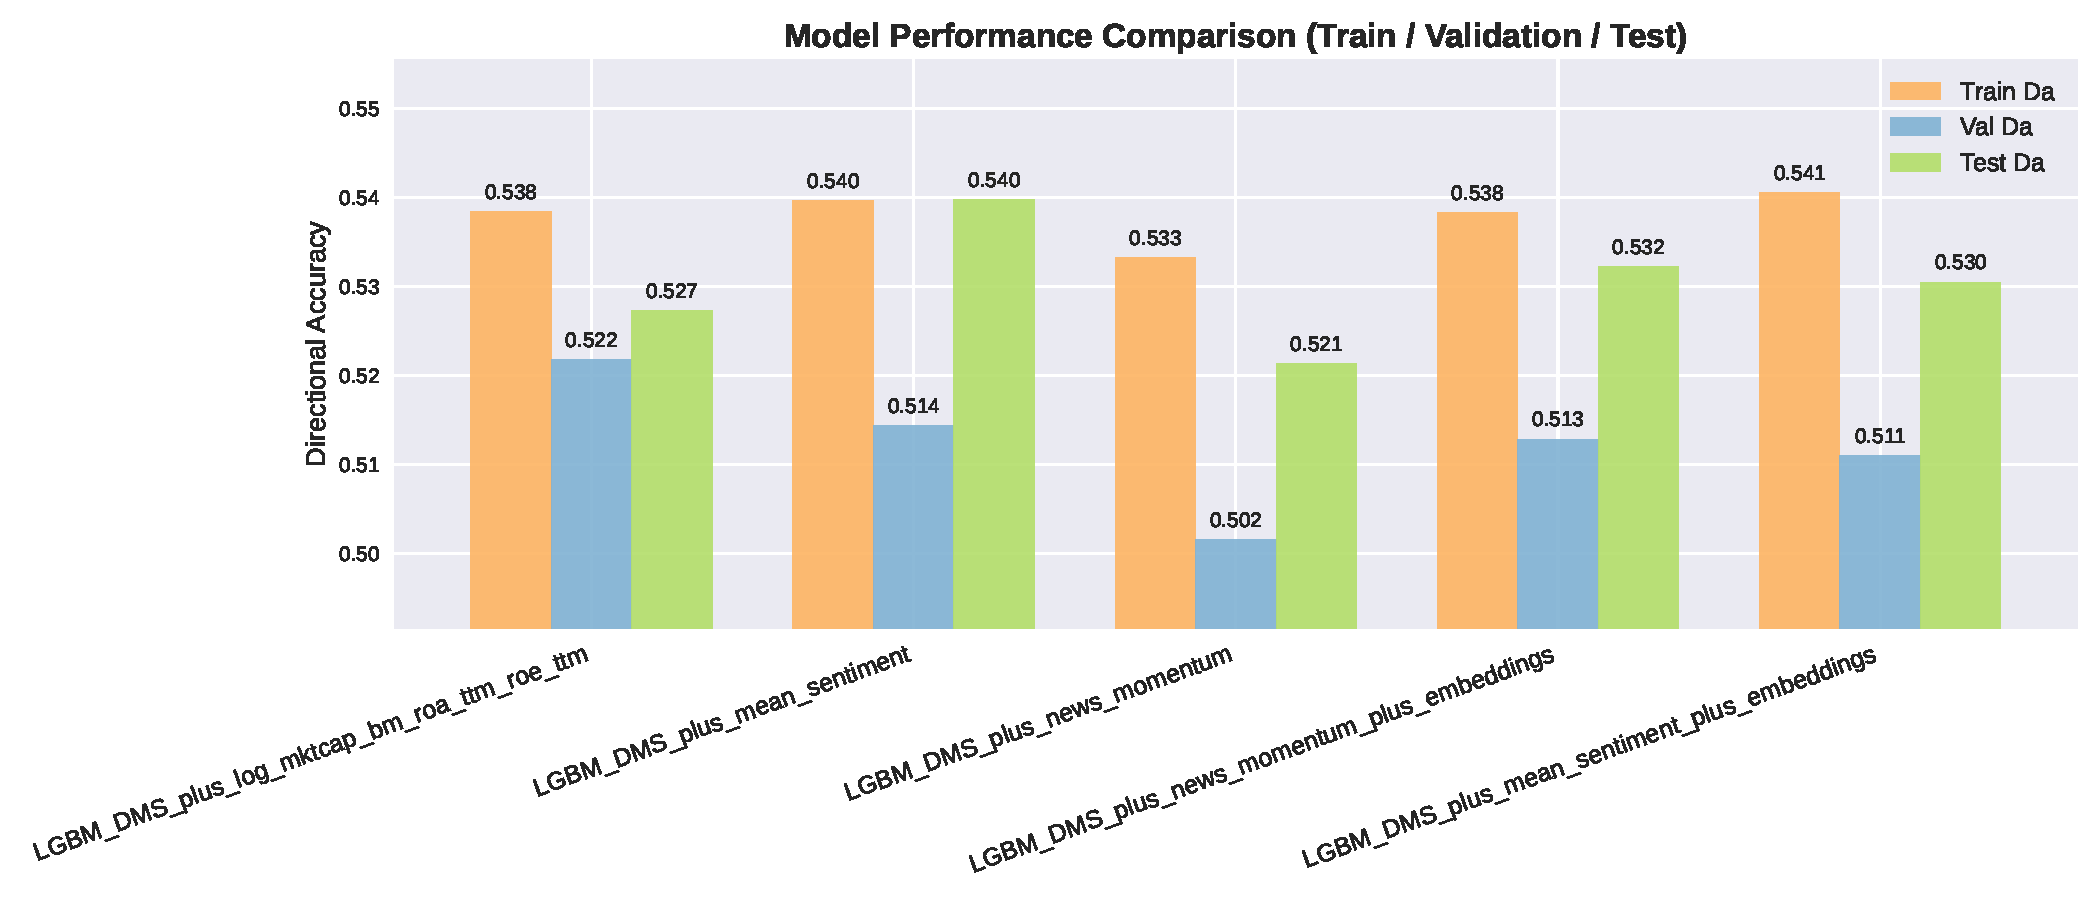
\includegraphics[width=0.8\linewidth]{../figures/model_performance_comparison.pdf}
    \caption{Directional accuracy for LightGBM models trained with different feature sets.}
    \label{fig:model_performance_comparison}
\end{figure}
\noindent \textbf{Interpretation.}  
Across all models, directional accuracy remains in the narrow range of $0.51$–$0.54$, consistent with well-known limits on daily return predictability. Several patterns emerge. First, all models outperform a naïve random-guessing benchmark (50\%), confirming that even simple tabular signals contain economically meaningful information. Second, the \textit{Fundamentals} and \textit{Mean Sentiment} models achieve the highest test accuracy (approximately $0.540$), indicating that slow-moving valuation ratios and high-level news sentiment indicators are the most stable predictors in our dataset. Third, adding PCA-based text embeddings does not improve performance and, in some cases, slightly reduces accuracy; this suggests that embeddings introduce additional noise relative to their marginal predictive value in daily horizons. Finally, the full \textit{News Momentum} feature set yields modest gains over mean sentiment alone, but the improvement is not consistently reflected on the validation and test splits, which indicates overfitting.  


\subsection*{Portfolio Performance under CVaR Optimization with Different Feature Sets}
\begin{figure}[H]
    \centering
    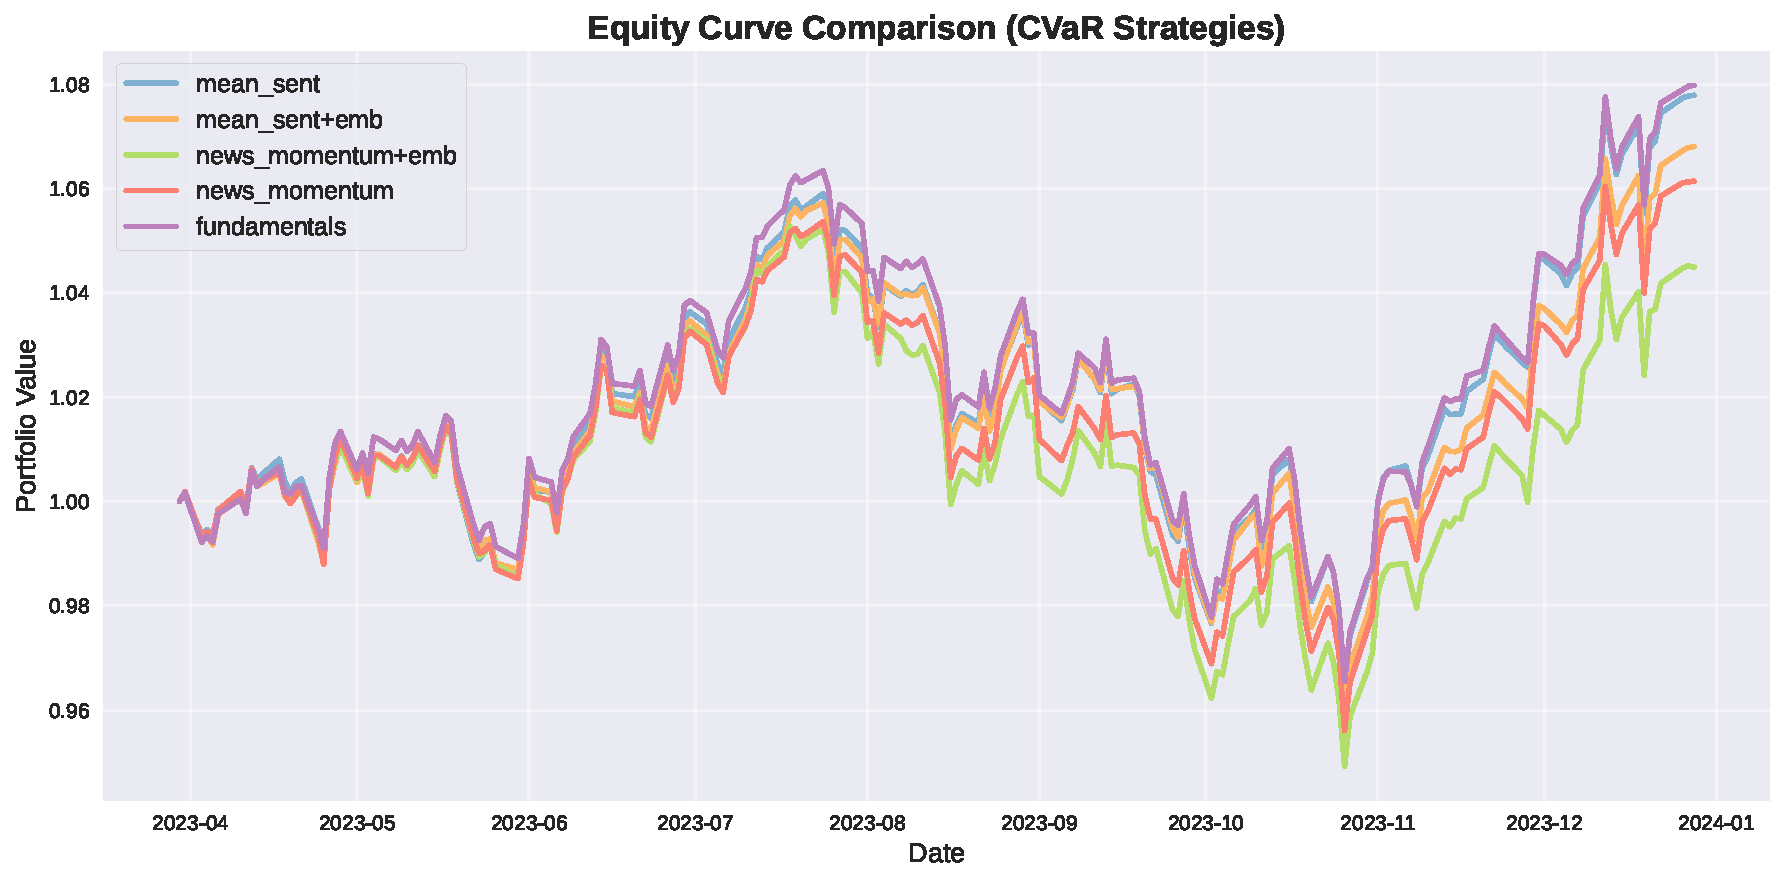
\includegraphics[width=0.8\linewidth]{../figures/cvar_equity_curves.pdf}
    \caption{Equity curves for portfolios using CVaR optimization with different feature sets.}
    \label{fig:cvar_equity_curves}
\end{figure}

\begin{table}[H]
\centering
\caption{Performance and Information Coefficient (IC) Statistics for Different Feature Sets}
\label{tab:performance_ic}
\begin{tabular}{lccccc}
\toprule
\textbf{Model} 
    & \textbf{Sharpe} 
    & \textbf{Ann. Return (\%)} 
    & \textbf{Mean IC} 
    & \textbf{IR} \\
\midrule

DMS + Fundamentals                 
    & \textbf{1.166} 
    & \textbf{10.84} 
    & \textbf{0.02834} 
    & \textbf{0.1669}  \\
DMS + Mean Sentiment               
    & \textbf{1.142} 
    & \textbf{10.58} 
    & \textbf{0.02685} 
    & \textbf{0.1691}  \\
DMS + Mean Sentiment + Embeddings  
    & 0.989 
    & 9.23 
    & 0.02067 
    & 0.1629  \\
DMS + News Momentum                
    & 0.895 
    & 8.32 
    & 0.02786 
    & 0.1906  \\

DMS + News Momentum + Embeddings   
    & 0.654 
    & 6.07 
    & 0.01457 
    & 0.1312  \\
\bottomrule
\end{tabular}
\end{table}
\noindent \textbf{Interpretation.}
Table~\ref{tab:performance_ic} summarizes both economic performance and statistical signal quality. The \textit{Sharpe ratio} and \textit{annualized return} reflect how well each model performs when translated into a trading strategy, while the \textit{Information Coefficient (IC)} measures the cross-sectional correlation between predicted and realized returns. The \textit{Information Ratio (IR)} indicates the stability of this signal over time.\\

\noindent Fundamentals and mean sentiment deliver the strongest performance, with the highest Sharpe ratios ($\approx 1.14$–$1.17$) and mean IC values ($\approx 0.027$–$0.028$). This suggests that slow-moving fundamentals and aggregate sentiment remain the most reliable predictors at a daily horizon. Adding text embeddings consistently reduces both Sharpe and IC, indicating that high-dimensional embeddings introduce noise rather than improving predictability. News momentum features offer moderate improvements in IC stability (higher IR) but do not outperform fundamentals in realized portfolio performance. Overall, simpler feature sets provide clearer and more stable signals than embedding-augmented models.


\section{Discussion and Conclusion}
\section{Contribution}

% \newpage
% \section*{Appendix}
\end{document}
